%+----------------------------------------------------------------------------+
%| SLIDES: template
%| Contents:	- x minutes (extimated duration 3 minutes per slide )
%|
%| Author: Antonio miti
%| Place: 
%| Date: 
%+----------------------------------------------------------------------------+


%- HandOut Flag -----------------------------------------------------------------------------------------
	\newif\ifHandout
	%\Handouttrue  %uncomment for the printable version
	%Handling of flags it is not preserved when passing to standalone-subfiles!


%- D0cum3nt ----------------------------------------------------------------------------------------------
\ifHandout
	\documentclass[handout,10pt]{beamer}   
	\setbeameroption{show notes} %print notes   
\else
	\documentclass[10pt]{beamer}
\fi




%- Packages ----------------------------------------------------------------------------------------------
\usepackage{custom-style}


%--Beamer Style-----------------------------------------------------------------------------------------------
\usetheme{toninus}


\usetikzlibrary{backgrounds}
  \tikzset{
    invisible/.style={opacity=0},
    visible on/.style={alt=#1{}{invisible}},
    alt/.code args={<#1>#2#3}{%
      \alt<#1>{\pgfkeysalso{#2}}{\pgfkeysalso{#3}} % \pgfkeysalso doesn't change the path
    },
  }



%- T1tle P4g3 -------------------------------------------------------------------------------------------
\title{
Gauge transformations of multisymplectic manifolds and $L_\infty$ observables
}
\subtitle{}
\author[AMM]{\href{https://dmf.unicatt.it/miti/}{Antonio Michele Miti}}
\institute[UCSC and KU Leuven]{
  \begin{tabular}[h]{ccc}
      Università Cattolica del Sacro Cuore & $\qquad$ & KU Leuven \\
      Brescia, Italy & & Leuven, Belgium \\
      \href{https://dipartimenti.unicatt.it/dmf-home?rdeLocaleAttr=it}{
\includegraphics[width=3.5cm]{Logos/UnicattBS-logo}} & & 
      \href{https://wis.kuleuven.be/english}{
\includegraphics[width=4cm]{Logos/KULeuven_logo}}
  \end{tabular}      
}
\date[Template_21] % (optional, should be abbreviation of conference name)
{	
	{\vskip 2ex}
	\href{https://public.eimi.ru/~cblacker/yrvmgc_21.html}{Young Researchers' Virtual Multisymplectic Geometry Workshop} \\
	{\vskip 1ex}
	Online, July 13, 2021
}





\newcommand{\thankyouslide}[0]{
	\ifHandout

	\else
	\addtocounter{framenumber}{-1}
	\begin{frame}{}
	\label{frame:thankyouslide}
		\vfill
	  \centering 
	  {\Huge\color{red} 
	  \emph{Thank you for your attention!}}
		\vfill
		%
		\centering
		\fbox{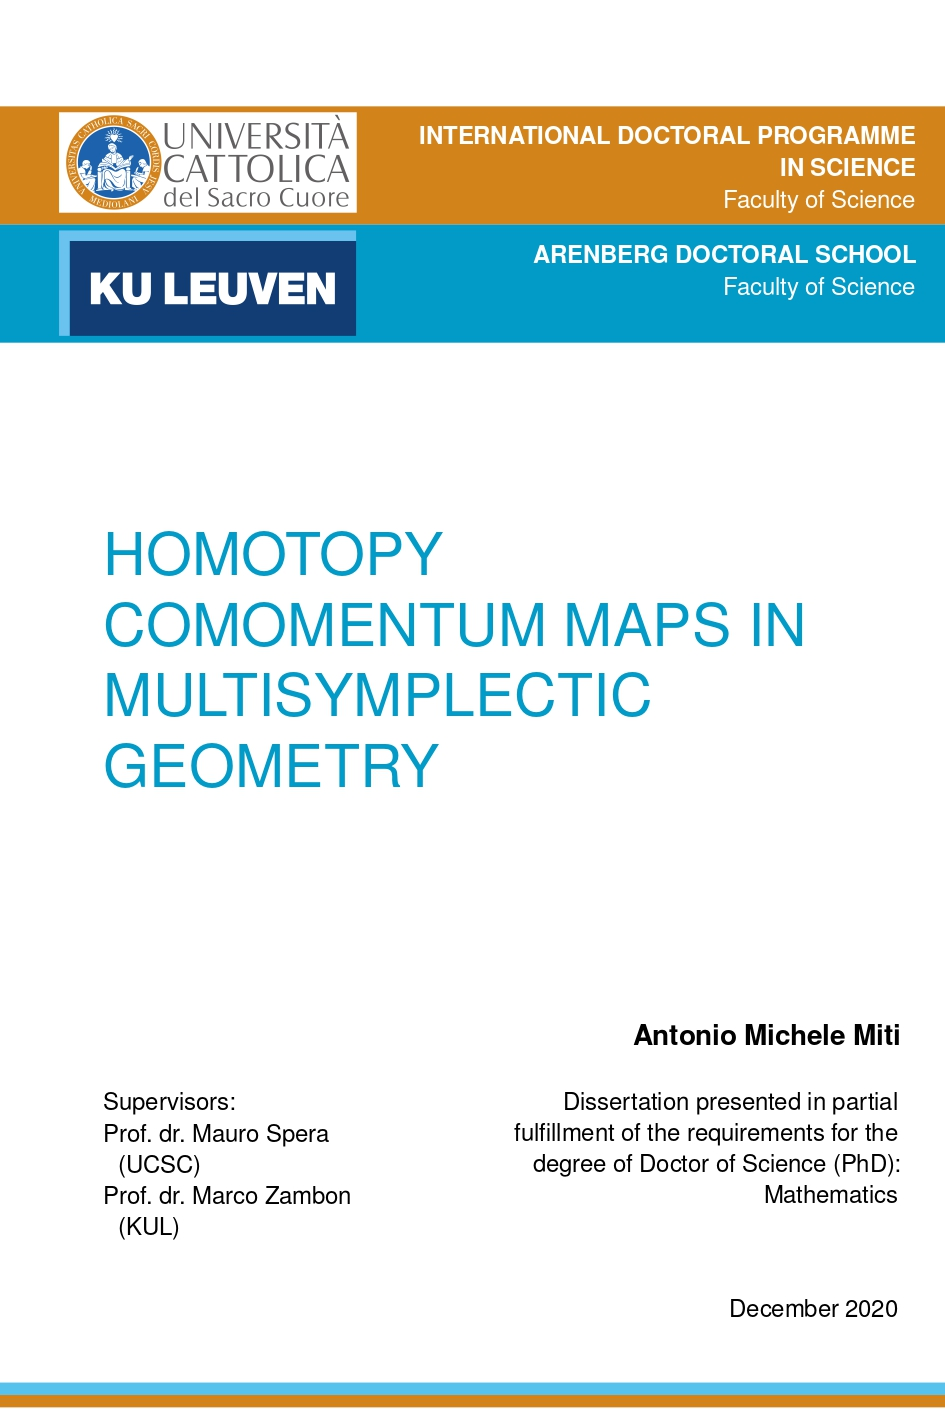
\includegraphics[width=.4\textwidth]{Pictures/thesis-cover}}
	\end{frame}
	\note[itemize]{
		\item
	}
	\fi
}






%---------------------------------------------------------------------------------------------------------------------------------------------------
%- D0cum3nt ----------------------------------------------------------------------------------------------------------------------------------
\begin{document}
%-------------------------------------------------------------------------------------------------------------------------------------------------
\begin{frame}  % Alternative: \maketitle outside of frame
	\titlepage
	\ifHandout
		\tikz[overlay,remember picture]
		{
	    	%	\node at ($(current page.west)+(1.5,0)$) [rotate=90] {\Huge\textcolor{gray}{\today}};
	    	\node[        
	    		draw,
	    		shape border rotate=90,
			isosceles triangle,
			isosceles triangle apex angle=90,
			fill=yellow]
	        		at ($(current page.north east)-(1,1)$) [rotate=-45] {\textcolor{red}{Handout version}};
		}
	\fi
	\end{frame}
	\addtocounter{framenumber}{-1}
\note{
	%\textbf{\underline{OUTLINE}}:
	%\tableofcontents
	\textbf{Abstract:}
	\\
Multisimplectic manifolds are a simple generalization of symplectic manifolds where closed non-degenerate k-forms are considered in place of 2-forms.
A natural theme that raises when dealing with both symplectic and multisymplectic structures is to investigate what relationship exists between gauge-related multisymplectic manifolds, i.e. endowed with multisymplectic forms lying in the same cohomology class.

In this talk, we will focus on the L-infinity algebras of observables associated to a pair of gauge related manifold.
To date, no canonical correspondence is known between two gauge-related observables algebras.
However, we will be able to exhibit a compatibility relation between those observables that are momenta of corresponding homotopy moment maps (the higher analogue of a moment map in the multisymplectic setting).

Although this construction is essentially algebraic in nature, it admits also a geometric interpretation when declined to the particular case of pre-quantizable symplectic forms. This provides some evidence that this construction may be related to the higher analogue of geometric quantization for integral multisymplectic forms.

This is ongoing joint work with Marco Zambon.
}
%---------------------------------------------------------------------------------------------------------------------------------------------------





%-------------------------------------------------------------------------------------------------------------------------------------------------
\section{Introduction}
%-------------------------------------------------------------------------------------------------------------------------------------------------
	%- HandOut Flag -----------------------------------------------------------------------------------------
\makeatletter
\@ifundefined{ifHandout}{%
  \expandafter\newif\csname ifHandout\endcsname
}{}
\makeatother

%- D0cum3nt ----------------------------------------------------------------------------------------------
\documentclass[beamer,10pt]{standalone}   
%\documentclass[beamer,10pt,handout]{standalone}  \Handouttrue  

\ifHandout
	\setbeameroption{show notes} %print notes   
\fi

	
%- Packages -------------------------------------------------------------------------------------------
\usepackage{custom-style}
\usetikzlibrary{positioning}
\usepackage{multicol}
\usepackage{stmaryrd}

%--Beamer Style----------------------------------------------------------------------------------------
\usetheme{toninus}
\usepackage{animate}
\usetikzlibrary{positioning, arrows}
\usetikzlibrary{shapes}

%--Custom command----------------------------------------------------------------------------------------
\providecommand{\pairing}{\langle\cdot,\cdot\rangle}
\providecommand{\vHam}{\mathscr{v}}

\begin{document}
\outline


%-------------------------------------------------------------------------------------------------------------------------------------------------
\subsection{(Multi)-symplectic: mechanical perspective}
%-------------------------------------------------------------------------------------------------------------------------------------------------
\begin{frame}{Symplectic geometry (mechanical perspective)}
\begin{columns}[T]
	\begin{column}{.50\linewidth}
		\centering
		\textit{ "geometric approach" to mechanics \dots}
		%
		\begin{columns}
			\begin{column}{.60\linewidth}
				\begin{center}
					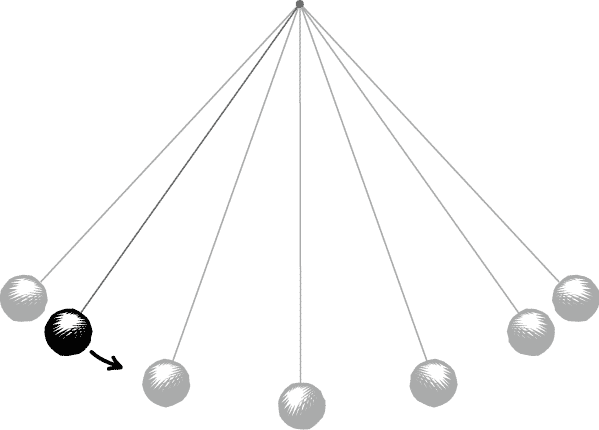
\includegraphics[width=0.6\linewidth]{Pictures/pendulum13}			
				\end{center}
			\end{column}	
			\begin{column}{.40\linewidth}
				\begin{center}
					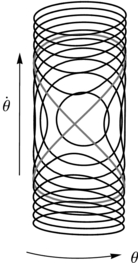
\includegraphics[width=0.45\linewidth]{Pictures/pendulum-phase-space}			
				\end{center}
			\end{column}	
		\end{columns}
		%
		\begin{defblock}[Symplectic Manifold]
			\vspace{-1em}
			\includestandalone[width=1\textwidth]{Pictures/Figure_sym}	
		\end{defblock}
		%
		\pause
		\begin{exblock}[$M = T^\ast Q$ is symplectic]
			with $\omega = d \theta $ given by
			$$ \left.\theta\right\vert_{(q,p)} (v) = p (\pi_\ast v) ~.$$
		\end{exblock}
		%
		\pause
		\vspace{1em}
		\centering
		\textit{ based on the notion of "states".}		
	\end{column}
	\onslide<1->{\vrule{}}
	\pause
	\begin{column}{.50\linewidth}
		\centering
		\textit{ "algebraic approach" to mechanics \dots}
		\vspace{.5em}	
		\begin{defblock}[Classical Observables]
			Unital, associative, commutative algebra $C^\infty(M)$.
		\end{defblock}
		%
		\vspace{.5em}
		\pause
		\begin{defblock}[Hamiltonian vector fields]
			$v_f \in \mathfrak{X}(M)$ such that:
			$$\iota_{v_f} \omega = -df \quad \text{(exact)}$$ %$\in B^1(M)$
			\small$v_f$ = \emph{Ham.v.f. pertaining to $f\in C^\infty(M)$}.
		\end{defblock}
		%
		\begin{defblock}[Poisson Algebra of Observables]
			$C^\infty(M)$ is a Poisson algebra with
			$$\{f,g\} = \iota_{v_g} \iota_{v_f} \omega = \omega(v_f,v_g) ~.$$
		\end{defblock}
		%
		\pause
		\vspace{.8em}
		\centering
		\textit{ based on the notion of "meaurable quantities".}						
	\end{column}
\end{columns}
\end{frame}
\note[itemize]{
	\footnotesize

	\item We work in the framework of multisymplectic geometry which is one of the possible generalizations of the well-established field of symplectic geometry.
	
	\item To recall what symplectic geometry is let me assume a particular point of view: mechanics.
	\\
	Idea:"
	Symplectic geometry is a branch of differential geometry studying symplectic manifolds; it originated as a formalization of the mathematical apparatus of classical mechanics and geometric optics."{\href{https://ncatlab.org/nlab/show/symplectic+geometry}{nlab}}
	
	Namely, a sym. mfd. is the geometric structure encoding the phase space of conservative, ordinary, classical, mechanical systems.
	
	\item $\theta$ = \emph{tautological 1-form}.
		$\theta$ evaluated at $p\in T^*Q$ in the fibre of $q\in Q$ and contracted with $v$ coincides with the form $p$ evaluated at $q$ and contracted with the push forward of $v$.
	
	\item We identify a special class of vector fields.
		Out of them one can define a Lie bracket.
	
	\item Poisson is a Lie algebra with the extra property of compatibility with the associative product (Leibniz rule)
	
	\item take away message: geometric (based on "states") vs algebraic (based on "measurable quantities").7
}
%-------------------------------------------------------------------------------------------------------------------------------------------------


%-------------------------------------------------------------------------------------------------------------------------------------------------
\begin{frame}[t]{From Symplectic to MultiSymplectic (mechanical perspective)}
	\begin{block}{Historical motivation}
		Mechanics: geometrical foundations of \textit{(first-order)} field theories.
		\begin{itemize}
		 \item[•] Kijowski, W. Tulczyjew \cite{Kijowski1979}; %(1979)
		 \item[•] Cariñena, Crampin, Ibort \cite{Carinena1991b};% (1991)
		 \item[•] Gotay, Isenberg, Marsden, Montgomery \cite{Gimmsy1};%(1998)
		 \\ $\cdots$
		\end{itemize}
	\end{block}
	\vfill
	\pause
	\tcbset{colback=white,
		colbacktitle=white,
		colframe=red!70!black,
		boxrule=1pt,
		colupper=red!70!black,
		arc=15pt}
	\begin{tcolorbox}[enhanced,frame hidden,borderline={0.5pt}{0pt}{red,dashed}]
		\color{red}
		\begin{columns}[T]
			\begin{column}{.20\linewidth}
				\begin{center}
					\huge
					\faWarning
				\end{center}
			\end{column}			
			\begin{column}{.60\linewidth}
				\vspace{-.4em}
				\begin{center}
					The lack of a satisfactory notion of observables hindered the spread of this formalism.
				\end{center}
			\end{column}			
			\begin{column}{.20\linewidth}
				\begin{center}
					\huge
					\faWarning
				\end{center}
			\end{column}			
		\end{columns}
	\end{tcolorbox}
	\vfill
	\pause
	\begin{tcolorbox}[enhanced,frame hidden,borderline={0.5pt}{0pt}{blue,dashed}]
		\color{blue}
		\begin{columns}[T]
			\begin{column}{.20\linewidth}
				\begin{center}
					\huge
					\faQuestionCircle
				\end{center}
			\end{column}			
			\begin{column}{.60\linewidth}
				\begin{center}
					\vspace{-.4em}
					{Why observables are so crucial?\qquad \qquad Quantization!}	
				\end{center}
			\end{column}			
			\begin{column}{.20\linewidth}
				\begin{center}
					\huge
					\faQuestionCircle
				\end{center}
			\end{column}			
		\end{columns}
	\end{tcolorbox}




\end{frame}
\note[itemize]{
	\item Historically, the interest in multisymplectic manifolds, has been motivated by the need for understanding the geometrical foundations of first-order classical field theories.
	The key point is that, just as one can associate a symplectic manifold to an ordinary classical mechanical system (e.g. a single
point-like particle constrained to some manifold), it is possible to associate a multisymplectic
manifold to any classical field system (e.g. a continuous medium like a filament or a fluid). See frame Extra-\ref{Frame:Ms-Field-Mechanics} 
	\item Forger and Romero say: \emph{"The multisymplectic formalism is manifestly consistent with the basic principles of field theory, preserving full covariance, and it is mathematically rigorous because it uses well established methods from calculus on finite-dimensional manifolds. On the other hand, it does not seem to permit any obvious definition of the Poisson bracket between observables. Even the question of what mathematical objects should represent physical observables is not totally clear and has in fact been the subject of much debate in the literature. Moreover, the introduction of n conjugate momenta for each coordinate obscures the usual duality between canonically con- jugate variables (such as momenta and positions), which plays a fundamental role in all known methods of quantization.A definite solution to these problems has yet to be found."}
	
}
%-------------------------------------------------------------------------------------------------------------------------------------------------

%-------------------------------------------------------------------------------------------------------------------------------------------------
\subsection{Observability}
%-------------------------------------------------------------------------------------------------------------------------------------------------
\begin{frame}{Observables in $n$-plectic geometry}
	%
	\begin{defblock}[Hamiltonian $(n-1)$-forms]
		\begin{displaymath}
			\Omega^{n-1}_{ham}(M,\omega) 	:=
			\biggr\{ \sigma \in  \Omega^{n-1}(M) \; \biggr\vert \; 
				\exists \vHam_\sigma \in \mathfrak{X}(M) ~:~ 
				\tikz[baseline,remember picture]{\node[rounded corners,
                        fill=orange!5,draw=orange!30,anchor=base]            
            			(target) {$d \sigma = -\iota_{\vHam_\sigma} \omega$ };
            	}				
				~\biggr\} 
			\end{displaymath}
	\end{defblock}

	\pause
		\tikz[overlay,remember picture]
		{
			\node[rounded corners,
                 fill=orange!5,draw=orange!30,anchor=base]
            	 (base) at ($(current page.north east)-(2,1)$) [rotate=-0,text width=3.5cm,align=center] {\footnotesize{\textcolor{red}{Hamilton-DeDonder-Weyl \\equation}}};
		}	
	\begin{tikzpicture}[overlay,remember picture]
    	\path[->] (base.south) edge[bend right,red](target.north);
    \end{tikzpicture}
	%
	\vspace{-2em}
	\begin{columns}[T]
		\pause
		\setlength{\belowdisplayskip}{5pt}
		\begin{column}{.50\linewidth}
			%
			\begin{thmblock}[Observables $L_\infty$-algebra]
				$\Omega^{n-1}_{ham}(M,\omega)$ endowed with
				\vspace{-.5em}
				\begin{displaymath}
					\lbrace \sigma_1, \sigma_2 \rbrace =			
					~ - \iota_{\vHam_1}\iota_{\vHam_2} \omega 
				\end{displaymath}			
				can be "completed" to a \\ $L_\infty-algebra$.
			\end{thmblock}
			%
			\pause
			\begin{itemize}
				\item[\cmark] Skew-symmetric;
				\item[\xmark] multiplication of observables;
				\item[\xmark] Jacobi equation;
				%\\ \hspace*{4.25em} full-fledged Jacobi equation;
				\item[\smark] Jacobi equation \emph{up to homotopies}.
			\end{itemize}				
		\end{column}	
		%
		\onslide<1->{\vrule{}}
		%
		\pause
		\begin{column}{.50\linewidth}
			\begin{thmblock}[Observables Leibniz algebra]
				$\Omega^{n-1}_{ham}(M,\omega)$ endowed with
				\vspace{-.5em}
			\begin{displaymath}
				\llbracket \sigma_1, \sigma_2 \rrbracket =
				~ \mathcal{L}_{\vHam_1} \sigma_2
				~.					
			\end{displaymath}		
				can be "completed" to a \\ DG-Leibniz algebra.
			\end{thmblock}	
			%
			\pause
			\begin{itemize}
				\item[\xmark] Skew-symmetric;
				\item[\xmark] multiplication of observables;
				\item[\cmark] Jacobi equation;
				\item[\smark] Skew-symmetric \emph{up to homotopies}.
			\end{itemize}	
		\end{column}	
	\end{columns}
\end{frame}
\note[itemize]{
 \item See \cite[\S 7.2]{Rogers2010} about the comparison of these two algebraic structures.
 \item Notice that the failure of skew-symmetricity is measured by
 \begin{align*}
 	A(\sigma_1,\sigma_2) 
 	=&~
 	 2~\llbracket \sigma_1, \sigma_2\rrbracket +  \llbracket \sigma_2, \sigma_1\rrbracket
 	 \\
 	 =&~ d \circ\langle\sigma_1,\sigma_2\rangle_+
 \end{align*}
 (Compare with the \href{https://en.wikipedia.org/wiki/Courant_bracket\#Dorfman_bracket}{Dorfmann bracket}.)
 
 \item Notice that the antisymmetrization of $\llbracket \cdot, \cdot \rrbracket$ equates $\lbrace \cdot,\cdot \rbrace$ modulo homotopy:
 \begin{align*}
  \llbracket \sigma_1,\sigma_2 \rrbracket  \circ 	\mathcal{A}
  =&~
  \frac{\mathcal{L}_{\vHam_1}\sigma_2 - \mathcal{L}_{\vHam_2}\sigma_1}{2} 
  \\
  =&~ 
  \frac{1}{2}( d (\iota_{\vHam_1}{\sigma_2} - \iota_{\vHam_2}{\sigma_1} )
  +\frac{1}{2}(-\iota_{\vHam_1}\iota_{\vHam_2}\omega + \iota_{\vHam_2}\iota_{\vHam_1}\omega) 
  \\
  =&~
  \lbrace \sigma_1, \sigma_2 \rbrace + d \circ \langle\sigma_1,\sigma_2\rangle_-
  \\
  =&~
  [\sigma_1,\sigma_2]_\omega
 \end{align*}
 where the last bracket is given by the Vinogradov algebroid Binary bracket.
}
%-------------------------------------------------------------------------------------------------------------------------------------------------

%------------------------------------------------------------------------------------------------------
\begin{frame}{Scope of the talk}
	%
	\centering
	\begin{tikzpicture}
		\node [draw,ellipse callout,red, minimum height=10em,minimum width=30em,callout relative pointer={(-2,-.5)}] (L1) {};
		\node [text width=25em,text centered] (L2) {
			\textcolor{red}{Broad \emph{general} question:}
			\\
			\medskip
			What is the corresponding	 "correct" notion of observables in multisymplectic geometry?	
		};
	\end{tikzpicture}
	\vfill
	\pause
	\begin{tikzpicture}
		\node [draw,blue,ellipse callout, minimum height=10em,minimum width=30em,callout relative pointer={(2,-.5)}] (L1) {};
		\node [text width=25em,text centered] (L2) {
			\textcolor{blue}{Specific \emph{technical} question}:
			\\
			\medskip
			How the compatibility diagram between \emph{gauge transformation}
			and \emph{comomentum maps} extends to the $n$-plectic case?
		};
	\end{tikzpicture}
\end{frame}
\note[itemize]{
	\item Non ho una risposta soddifacente alla domanda generale. Bisogna procedere per gradi.
	\item l'obbiettivo di questo lavoro con Marco è di stabilire quanto della seguente situazione si estende nel caso multisimplettico.
	\item It is possible to relate the observables algebras of two gauge-related multisymplectic structures (in he same cohomology class)
}
%-------------------------------------------------------------------------------------------------------------------------------------------------



\end{document}




%-------------------------------------------------------------------------------------------------------------------------------------------------
\section{Gauge Compatibility Problem - Symplectic Case}
\checkpoint	
%-------------------------------------------------------------------------------------------------------------------------------------------------
	%- HandOut Flag -----------------------------------------------------------------------------------------
\makeatletter
\@ifundefined{ifHandout}{%
  \expandafter\newif\csname ifHandout\endcsname
}{}
\makeatother

%- D0cum3nt ----------------------------------------------------------------------------------------------
\documentclass[beamer,10pt]{standalone}   
%\documentclass[beamer,10pt,handout]{standalone}  \Handouttrue  

\ifHandout
	\setbeameroption{show notes} %print notes   
\fi

	
%- Packages ----------------------------------------------------------------------------------------------
\usepackage{custom-style}
\usetikzlibrary{positioning}
\usepackage{multicol}


%--Beamer Style-----------------------------------------------------------------------------------------------
\usetheme{toninus}
\usepackage{animate}
\usetikzlibrary{positioning, arrows}
\usetikzlibrary{shapes}

\begin{document}
%-------------------------------------------------------------------------------------------------------------------------------------------------


%-------------------------------------------------------------------------------------------------------------------------------------------------
\subsection{Poisson algebra and Lie algebroids}
%-------------------------------------------------------------------------------------------------------------------------------------------------
%-------------------------------------------------------------------------------------------------------------------------------------------------
\begin{frame}[fragile]{Embedding of the observables algebra in the Lie algebroid}
	Given a \alert{symplectic mfd.} $(M,\omega)$ ...
	\vfill
	\begin{center}
		\includestandalone[width=.95\textwidth]{Pictures/Frame_Embedding_Diagram_symplectic}
	\end{center}
	\vfill
	\begin{minipage}[t][8.5em][t]{\textwidth}
		\begin{itemize}
			\only<1-3>{
			\item<1-> \alert<1>{... there is a naturally associated Poisson algebra ...}
			\item<2-> \alert<2>{... and also a (standard twisted) Lie Algebroid}.
			\item<3-> A Lie algebroid is a "controlled" $\infty$-dimensional Lie algebra given (in this case) by
			\begin{displaymath}
					\left[\binom{x_1}{f_1},\binom{x_2}{f_2}\right]
					~=~
					\binom{[x_1,x_2]}{x_1(f_2)-x_2(f_1)-\omega(x_1,x_2)}
				\end{displaymath}
			}
			\item[]<4->
				\quad\\
				\begin{thmblock}[There exists an embedding of Lie algebras.]
					\begin{displaymath}
						\begin{tikzcd}
							\Psi~:&[-1em] C^{\infty}(M)_\omega \ar[r,"\Psi"]& \Gamma(TM\oplus \mathbb{R})_\omega
							\\[-2em]
							& f \ar[r,mapsto] & \binom{\mathscr{v}_f}{f}
						\end{tikzcd}		
					\end{displaymath}
				\end{thmblock}
		\end{itemize}
	\end{minipage}
\end{frame}
\note{}
%-------------------------------------------------------------------------------------------------------------------------------------------------


%-------------------------------------------------------------------------------------------------------------------------------------------------
\subsection{Compatibility between gauge transformations}
%-------------------------------------------------------------------------------------------------------------------------------------------------
%-------------------------------------------------------------------------------------------------------------------------------------------------
\begin{frame}[fragile]{Compatibility between gauge transformations and comoment maps}
	%
	Consider $(M,\omega)$ \alert{symplectic mfd.}
	%
	\begin{center}
			\includestandalone[width=.8\textwidth]{Pictures/Frame_BigDiagram_symplectic}
	\end{center}
	%
	\vspace{-1em}
	\vfill
	\begin{minipage}[t][8em][t]{\textwidth}
		\begin{itemize}
			\only<2>{
				\item<2-> Consider a second gauge-related symplectic structure on $M$
					\begin{displaymath}
						\tilde{\omega} = \omega + d B \qquad \text{with} \quad B\in \Omega^1(M).
					\end{displaymath}
			}
			\only<3-4>{
				\item<3-> There is a natural isomorphism in the Lie Alg.oids category \emph{($B$-transformation)}
					\begin{displaymath}
						\binom{x}{f} \mapsto \binom{x}{f-\iota_x B} ~.
					\end{displaymath}
			}
			\only<6-7>{
				\item<6-> Consider an infinitesimal group action $\mathfrak{g}\circlearrowleft M$ which is Hamiltonian w.r.t. both $\omega$ and $\tilde{\omega}$.
				\item<7-> let be $f:\mathfrak{g} \to C^\infty(M)_\omega$ and $\tilde{f}:\mathfrak{g} \to C^\infty(M)_{\tilde{\omega}}$ two comoment map s.t.
				\begin{displaymath}
					\tilde{f}(\xi) = f(\xi) - \iota_{\underline{\xi}}B
				\end{displaymath}
				}
			\item[]						
		\end{itemize}
	\only<5>{
		\vspace{-.75em}
		\begin{center}
		\tcbox[enhanced,frame hidden,borderline={0.5pt}{0pt}{red,dashed}]{	
			\alert{
			\faQuestionCircle \qquad
				{How can we close the left-hand side?}
			\qquad \faQuestionCircle		
			}
		}
		\end{center}
	}
	\only<8->{
		\vspace{-.75em}
		\tcbset{colback=white,
		colbacktitle=white,
		colframe=red!70!black,
		boxrule=1pt,
		colupper=red!70!black,
		arc=15pt,
		}
		\begin{tcolorbox}[enhanced,frame hidden,borderline={0.5pt}{0pt}{blue}]
			\color{blue}{
			Lemma: The central pentagon commutes!
			}
		\end{tcolorbox}
	\vfill
	}
	\only<9->{
		\vspace{-.75em}
		\begin{center}
		\tcbox[enhanced,frame hidden,borderline={0.5pt}{0pt}{red,dashed}]{	
			\alert{
			\faQuestionCircle \qquad
				{What happens in the higher (n-plectic) case?}
			\qquad \faQuestionCircle		
			}
		}
		\end{center}
	}
	\end{minipage}	
\end{frame}
\note[itemize]{
	\item The horizontal embedding is  $f \mapsto (v_f,f)$;
	\item Vertical maps are also known as \emph{Gauge transformations}
	\item upshot: 
	\begin{enumerate}
		\item 
	\end{enumerate}
}
%-------------------------------------------------------------------------------------------------------------------------------------------------



%-------------------------------------------------------------------------------------------------------------------------------------------------
\subsection{Geometric interpretation in pre-quantization}
%-------------------------------------------------------------------------------------------------------------------------------------------------
%-------------------------------------------------------------------------------------------------------------------------------------------------
\begin{frame}[fragile]{Geometric interpretation of the diagram}
	%
	Consider $(M,\omega)$ \alert{symplectic} and \alert{\underline{prequantizable}}.
	%
	\begin{center}
			\includestandalone[width=.8\textwidth]{Pictures/Frame_BigDiagram_prequantum}
	\end{center}
	%
	\vspace{-2em}
	\begin{minipage}[t][1.7cm][t]{\textwidth}
	\begin{itemize}
		\only<1-3>{
			\item<1-> Fix a Prequantization Bundle $S^1\hookrightarrow P \to M$ with connection $\theta$,
			\item<2-> "infinitesimal quantomorphisms" $Q(P,\theta):=\lbrace Y \in \mathfrak{X}(P)~|~ \mathcal{L}_Y \theta =0 \}$.
		}
		\item<4-> Embdedding through Atiah algebroid.
	\end{itemize}
	\end{minipage}
	\vfill
	\tcbset{colback=white,
	colbacktitle=white,
	colframe=red!70!black,
	boxrule=1pt,
	colupper=red!70!black,
	arc=15pt,
	}
	\begin{minipage}[t][1.7cm][t]{\textwidth}
	\only<3>{ 
		\begin{tcolorbox}[enhanced,frame hidden,borderline={0.5pt}{0pt}{blue}]
			\color{blue}{
			Lemma: The left square commutes!
			}
		\end{tcolorbox}
	}
	\only<5>{
		\begin{tcolorbox}[enhanced,frame hidden,borderline={0.5pt}{0pt}{blue}]
			\color{blue}{
			Lemma: The left square and right triangle commute!
			}
		\end{tcolorbox}
	}
	\end{minipage}
	%
\end{frame}
\note[itemize]{
	\item questo fatto puramente algebrico ha un'interessante interpretazione nell'ambito della prequantizzaazione  Relevance to Prequantization
	\item The horizontal embedding is  $f \mapsto (v_f,f)$;
	\item Vertical maps are also known as \emph{Gauge transformations}
	\item upshot: 
	\begin{enumerate}
		\item 
	\end{enumerate}
}
%-------------------------------------------------------------------------------------------------------------------------------------------------


\end{document}


%-------------------------------------------------------------------------------------------------------------------------------------------------




\end{document}





%-------------------------------------------------------------------------------------------------------------------------------------------------
\section{Gauge Compatibility Problem - MULTISymplectic Case}
\checkpoint	
%-------------------------------------------------------------------------------------------------------------------------------------------------
	%- HandOut Flag -----------------------------------------------------------------------------------------
\makeatletter
\@ifundefined{ifHandout}{%
  \expandafter\newif\csname ifHandout\endcsname
}{}
\makeatother

%- D0cum3nt ----------------------------------------------------------------------------------------------
\documentclass[beamer,10pt]{standalone}   
%\documentclass[beamer,10pt,handout]{standalone}  \Handouttrue  

\ifHandout
	\setbeameroption{show notes} %print notes   
\fi

	
%- Packages ----------------------------------------------------------------------------------------------
\usepackage{custom-style}
\usetikzlibrary{positioning}
\usepackage{multicol}
\DeclareMathOperator{\varv}{\mathscr{v}}


%--Beamer Style-----------------------------------------------------------------------------------------------
\usetheme{toninus}
\usepackage{animate}
\usetikzlibrary{positioning, arrows}
\usetikzlibrary{shapes}

\begin{document}
%-------------------------------------------------------------------------------------------------------------------------------------------------

%---------------------------------------------------------------------------------------------------------------------------------------------------
\subsection{Lie $\infty$-algebra of Observables}
\begin{frame}[fragile,t]{Lie $\infty$-algebra of Observables (higher observables) }
	Let be $(M,\omega)$ a $n$-plectic manifold.
	\begin{defblock}[$L_\infty$-algebra of observables ~\emph{(Rogers)}]
		\hspace{.25em} Is a cochain-complex $(L,\{\cdot\}_1)$ \\
		\vspace{-2.5em}
		\begin{center}
		\ifHandout
			\includestandalone{Pictures/Figure_Observables}	
		\else
			\includestandalone{Pictures/Frame_Observables}
		\fi				
		\end{center}
		\onslide<2->{
			\hspace{.25em} with $n$ (skew-symmetric) multibrackets $(2 \leq k \leq n+1)$\\
			\vspace{-1.5em}
			\begin{center}
				\includestandalone{Pictures/Equation_Multibracket}	
			\end{center}
		}
		%
	\end{defblock}
  	\vfill
	\onslide<3->{
		\emph{Higher analogue} of the \emph{Poisson algebra structure} associated to a symplectic mfd.
	\vfill
	\begin{columns}
		\hfill
		\begin{column}{.11\linewidth}	
			If $n>1$:
			
		\end{column}	
		\begin{column}{.8\linewidth}
		\begin{itemize}
			\item[\xmark] \textcolor{red}{we lose} :\quad multiplication of observables, Jacobi equation;
			%\\ \hspace*{4.25em} full-fledged Jacobi equation;
			\item[\cmark] \textcolor{green}{we gain} :\quad brackets with arities different than two,\\
			\hspace*{4.25em}
			 Jacobi equation \emph{up to homotopies}.
		\end{itemize}		
		\end{column}		
	\end{columns}
	}
  \end{frame}
 \note[itemize]{
	\item if symplectic manifolds are the symmetric take on mechanics, Poisson algebras are the algebraic counterpart.
 	\item A Lie algebra is associated to an ordinary symplectic manifold (its Poisson algebra).
	%(Underlying this is a Lie algebra, whose Lie bracket is the Poisson bracket.)
	Similarly, one associates an Lie-$n$ algebra to any $n$-plectic manifold.
 	% https://ncatlab.org/nlab/show/n-plectic+geometry 	 
 	 %https://ncatlab.org/nlab/show/Poisson+bracket+Lie+n-algebra
	 \item Basically, the higher observables algebra is a chunk of the de Rham complex of $M$ with inverted grading( convention employed here) and an extra structure called "multibrackets".
 	\item ( In the 1-plectic case it reduces to the corresponding Poisson algebra of classical observables)
 	\item Rogers associated to any n-plectic mfd a $L\-\infty$ algebra, Zambon generalized it to the pre-n-plectic case.
 	\item Recognize in the definition of $\{\cdot,\ldots,\cdot\}_k$ the contraction with hamiltonian fields $v_\sigma$ w.r.t. $\sigma$.
  	\item Note $	\iota_{v_{\sigma_1}}\cdots\iota_{v_{\sigma_k}} = (-)^{(k-1)+(k-2)+\dots+1}\iota_{v_{\sigma_k}}\cdots\iota_{v_{\sigma_1}} = (-)^{\frac{k(k-1)}{2}}\iota_{v_{\sigma_k}}\cdots\iota_{v_{\sigma_1}}$ 
 	The definition usually find in literature of Rogers multibrackets involves the coefficient $ (-)^{\frac{k(k-1)}{2}} = -\varsigma(k-1) = (-)^{k+1} \varsigma(k)$.
  \item higher observables is Special instance of a more general object  called $L\-\infty$ Algebra...
 }
%------------------------------------------------------------------------------------------------


%-------------------------------------------------------------------------------------------------------------------------------------------------
\subsection{Homotopy comomentum maps}\label{frame:hcmm-main}
\begin{frame}[fragile]{Homotopy comomentum maps}
	Consider a Lie algebra action $v:\mathfrak{g} \to \mathfrak{X}(M)$  \underline{preserving the $n$-plectic form $\omega$}.
	\vfill
	\begin{defblock}[Homotopy comomentum map \emph{(Callies, Fregier, Rogers, Zambon)}]
		\ifHandout
			\includestandalone{Pictures/Figure_Lifting}
		\else
			\includestandalone{Pictures/Frame_Lifting}
		\fi					
	\end{defblock}
	\onslide<4->{
	\begin{lemblock}[HCMM unfolded  \cite{Callies2016}]
			%
			HCMM is a sequence of (graded-skew) multilinear maps:
			\begin{displaymath}
				(f)  = \big\lbrace f_k: \; \Lambda^k{\mathfrak g} \to L^{1-k} \subseteq \Omega^{n-k}(M) 
				~\big\vert~ 0\leq k \leq n+1  \big\rbrace
			\end{displaymath}
			\emph{fulfilling:}%\emph{such that:}
			\begin{itemize}
				\item<5-> $f_0 = 0 $, $f_{n+1} = 0$
				\item<6-> $d f_k (p) = f_{k-1} (
				\tikz[baseline,remember picture]{\node[rounded corners,
                        fill=green!5,draw=green!30,anchor=base]            
            			(target) {$\partial $ };
            	}				
				p)  - (-1)^{\frac{k(k+1)}{2}} \iota(v_p) \omega 
				\qquad\scriptstyle \forall p \in \Lambda^k(\mathfrak{g}),\; \forall k=1,\dots n+1$
			\end{itemize}
		\onslide<7->{
			\tikz[overlay,remember picture]
			{
				\node[rounded corners,
	                 draw=green!30,anchor=base]            
	            	 (base) at ($(current page.east)-(3,3)$) [rotate=-0,align=center] {\footnotesize{\hyperlink{frame:CE-complex}{\emph{Chevalley-Eilenberg boundary op.}}}};
			}	
		\begin{tikzpicture}[overlay,remember picture]
	    	\path[->] (base.west) edge[bend right,green](target.north east);
	    \end{tikzpicture}
	    }
	\end{lemblock}	
	}
	\vfill
\end{frame}
\note[itemize]{
	\item  An infinitesimal symmetry is a lie algebra morphism such that $\mathcal{L}_{v_x} \omega = 0 ~ \forall x \in \mathfrak{g}$.
	\\ (It is also call an infinitesimal multisymplectic action and $v_x$ is the infinitesimal generator of the action, corresponding to $x \in \mathfrak g$.) 
	\item Essentially, admitting a comoment maps mean that $v$ acts via Hamiltonian vector fields.
	\item In mechanical terms, a moment map is a tool associated with a Hamiltonian action of a Lie group on a symplectic manifold, used to construct conserved quantities for the action.(see \ref{frame:HCMMandConserved} in appendix.
}
%-------------------------------------------------------------------------------------------------------------------------------------------------

%-------------------------------------------------------------------------------------------------------------------------------------------------
\subsection{Vinogradov Algebroids}
%-------------------------------------------------------------------------------------------------------------------------------------------------
\begin{frame}{Vinogradov Algebroids}
	\begin{defblock}[Vinogradov algebroid (higher Courant)]
		\includestandalone[width=0.95\textwidth]{Pictures/Figure_vinogradov}	
	\end{defblock}

	\begin{itemize}
		\item $(n=1) ~ \Rightarrow$ standard twisted \emph{Lie algebroid};
		\item $(n=2) ~ \Rightarrow$ standard twisted \emph{Courant algebroid};
	\end{itemize}

\end{frame}
\note[itemize]{
\item Att, questa definizione sarebbe lo standard twisted. E' possibile trovare in letteratura definizioni piu' generali corrispondenti alla nozione di Courant algebroid in astratto.
}
%-------------------------------------------------------------------------------------------------------------------------------------------------

%-------------------------------------------------------------------------------------------------------------------------------------------------
\begin{frame}{Vinogradov $L_\infty$-algebra}
	Vin. alg.oids are $NQ$-manifolds ($L_\infty$-algebroids).
	$\quad\Rightarrow\quad$ 
	Associated $L_\infty$-algebra.

	\begin{defblock}[Vinogradov $L_\infty$-algebra \cite{Zambon2012}]
		\includestandalone[width=0.95\textwidth]{Pictures/Figure_vinogradov-Linfty}	
	\end{defblock}
	\vfill
	\only<6->{
		\tikz[overlay,remember picture]
		{
			\node[rounded corners,
                 fill=gray!1,draw=gray!30,anchor=base]            
            	 (base) at ($(current page.south)+(0,.5)$) [rotate=-0,text width=10cm,align=center] { \footnotesize{\color{gray}{
            	 $e_i = \pair{X_i}{\alpha_i} \in \mathfrak{X}(M)\oplus \Omega^{n-1}(M)$ 
            	 \quad~,\qquad
            	 $f_i \in \bigoplus_{k=0}^{n-2}\Omega^k(M)$.
            	 }}};
		}			
	}

\end{frame}
\note[itemize]{
	\item The actions of non vanishing multi-brackets (up to permutations of the entries) on arbitrary vectors
are given in the slide.
	\item $\mu_2 \left(e_1,e_2\right) 	= [e_1,e_2]_\omega 
			= \pair{[X_1,X_2]}{\dd \langle e_1, e_2\rangle_- 
			+ (\iota_{X_1}\dd\alpha_2 - \iota_{X_2}\dd\alpha_1 + \iota_{X_1}\iota_{X_2}\omega)}$
	\item $				\mu_2 \left(e_1,f_2\right) = -\mu_2(f_2,e_1) = 
				\frac{1}{2} \mathcal{L}_{X_1} f_2 = \langle e_1, \dd f_2 \rangle_-$
	\item $k$-ary bracket for $k \ge 3$ an \emph{odd} integer:	 
		\begin{equation}\label{eq:VinoMultibrakAllaZambon_1}
			\begin{split}
				\mu_k(\varv_0,\cdots,\varv_{k-1})
				=&
				\left(\sum_{i=0}^{k-1} {(-)^{i-1}\mu_k(f_i+\alpha_i,X_0,\dots,\widehat{X_i},\dots,X_{k-1})}\right)
				+\\
				&+(-)^{\frac{k+1}{2}} \cdot k \cdot B_{k-1} \cdot 
				\iota_{X_{k-1}}	\dots \iota_{X_{0}} \omega			
				~;
			\end{split}
		\end{equation}
		where 
		\begin{equation}\label{eq:VinoMultibrakAllaZambon_2}
			\begin{split}
			\mu_k&(f_0+\alpha_0,X_1,\dots,X_{n-1}) =
			\\
			&=
			~c_k
			\sum_{1\le i<j\le k-1}(-1)^{i+j+1}\iota_{X_{k-1}}\dots   
  			\widehat{\iota_{X_{j}}}\dots \widehat{\iota_{X_{i}}}\dots
				\iota_{X_{1}} ~ [f_0+\alpha_0,X_i,X_j]_3~.
			\end{split}
		\end{equation}			
In the above formula,		$[\cdot,\cdot,\cdot]_3 = -T_0$ denotes the ternary bracket %$\mu_3$ 
associated to the untwisted ($\omega=0$) Vinogradov Algebroid, and $c_k$ is a numerical constant
		\begin{equation}\label{eq:UglyCoefficient}
			c_k= (-)^{\frac{k+1}{2}}\frac{12~B_{k-1}}{(k-1)(k-2)}.
		\end{equation}
}
%-------------------------------------------------------------------------------------------------------------------------------------------------


%-------------------------------------------------------------------------------------------------------------------------------------------------
\subsection{Rogers embedding}
%-------------------------------------------------------------------------------------------------------------------------------------------------
\begin{frame}[fragile,t]{Embedding observables $L_\infty$-algebra into Vinogradov $L_\infty$-algebra}
	Consider now $\omega$ \alert{$n$-plectic}
	\vfill
	\begin{center}
		\includestandalone[width=.8\textwidth]{Pictures/Frame_Embedding_Diagram_k-plectic_V1}
	\end{center}
	\vfill
	\begin{minipage}[t][8.5em][t]{\textwidth}
	\only<4->{
	\begin{thmblock}[Embedding of $L_\infty$-algebras  $\Psi:L_\infty(M,\omega)\hookrightarrow L_{\infty}(E^n,\omega)$\quad \cite{Miti2021}.]
	\begin{itemize}[leftmargin=0pt]
		\item[$\cdot$]<4-> 
			consider the graded vector subspace $\mathcal{A}$
			\begin{displaymath}
			\mathclap{
			{\mathcal{A}^k} =
			\begin{cases}
		\left.\left\lbrace
		\binom{X}{\alpha}\in \mathfrak{X}(M)\oplus \Omega^{n-1}(M)
		~ \right\vert ~
		\iota_X \omega = -d \alpha\right\rbrace
&\quad k=0,\\
				\Omega^{n-1+k}(M) &\quad -n+1 \leq k < 0.
			\end{cases}			
			}
			\end{displaymath}						
		\item[$\cdot$]<5-> 
			restrict the two $L_\infty$-structures to $\pi$ and $\mu$ on $\mathcal{A}$
		\item[$\cdot$]<6->

			$L_\infty(M,\omega) \cong 
				(\mathcal{A},\pi) \color{blue}\cong\color{black}
				(\mathcal{A},\mu) \hookrightarrow
				L_\infty(E^n,\omega)$
	\end{itemize}
	\end{thmblock}
	}
	\only<6->{
		\tikz[overlay,remember picture]
		{
			\node[rounded corners,
                 fill=orange!1,draw=orange!30,anchor=base]            
            	 (base) at ($(current page.east)-(2.25,4)$) [rotate=-0,text width=3cm,align=center] { \footnotesize{\color{red}{
            	 Complete proof\\
            	 \faWarning ~ up to $n\geq 4$! ~ \faWarning 
            	 }}};
		}			
	}
	\end{minipage}
\end{frame}
\note[itemize]{
	\item this is the "work in progress" part of the preprint.
	\begin{itemize}
		\item[-] In the 1-plectic case is extremely simple to check.
		\item[-] The 2-plectic case has been constructed by Rogers in \cite{Rogers2010}.
		\item[-] Argument about existence by Ritter and Saemann \cite{Ritter2015}.
	\end{itemize}
}
%-------------------------------------------------------------------------------------------------------------------------------------------------


\subsection{Compatibility with Gauge transformations}
%-------------------------------------------------------------------------------------------------------------------------------------------------
\begin{frame}{Compatibility with Gauge transformations}
	Consider now $\omega$ \alert{n-plectic} \quad and \alert{$\tilde{\omega}=\omega + d B$}:
	\vfill
	%
	\begin{center}
		\includestandalone[width=.8\textwidth]{Pictures/Frame_Gauge_Diagram_k-plectic}
	\end{center}	
	%
	\vfill
	%
	

	\begin{itemize}
	\only<1-3>{
		\item<2-> Vinogradov alg.oids w.r.t cohomologous twisting closed forms are isomorphic.
		\item<3-> Induced isomorphism at the level of $L_\infty$-algebras
	}
	\only<4->{
		\item<4-> Consider a Lie algebra action $\mathfrak{g}\to \mathfrak{X}(M)$ admitting HCMM w.r.t $\omega$ and $\tilde{\omega}$
	}
	\end{itemize}

	\vfill
	\tcbset{colback=white,
		colbacktitle=white,
		colframe=blue!70!black,
		boxrule=1pt,
		colupper=blue!70!black,
		arc=15pt,
		}
	\onslide<5->{
	\begin{tcolorbox}[sidebyside,righthand width=.75\linewidth]
		Thm: \cite{Miti2021}
		\tcblower
		\color{blue}
The central square commutes. 
			\\\emph{(On the nose, not "up to homotopies")}.
	\end{tcolorbox}	
		\tikz[overlay,remember picture]
		{
			\node[rounded corners,
                 fill=orange!1,draw=orange!30,anchor=base]            
            	 (base) at ($(current page.east)-(1.75,4)$) [rotate=-0,text width=3cm,align=center] { \footnotesize{\color{red}{
            	 Complete proof\\
            	 \faWarning ~ up to $n\geq 4$! ~ \faWarning 
            	 }}};
		}		
	
	
	}
	

\end{frame}
\note[itemize]{
	\item Our results can be seen as a tiny step toward  undestanding the analogue of prequantization in the setting of multisymplectic geometry (hence field theory).
}
%-------------------------------------------------------------------------------------------------------------------------------------------------









%-------------------------------------------------------------------------------------------------------------------------------------------------
\end{document}





%-------------------------------------------------------------------------------------------------------------------------------------------------
	\thankyouslide
%------------------------------------------------------------------------------------------------



%------------------------------------------------------------------------------------------------
% APPENDIX
%------------------------------------------------------------------------------------------------
\appendix
%-------------------------------------------------------------------------------------------------------------------------------------------------
\section{Complementary Material}
	%+----------------------------------------------------------------------------+
%| SLIDES: 
%| Chapter: Complementary material - details on eventual questions
%| Author: Antonio miti
%| Event: PHD preliminary Defence
%+----------------------------------------------------------------------------+

%- HandOut Flag -----------------------------------------------------------------------------------------
\newif\ifHandout

%- D0cum3nt ----------------------------------------------------------------------------------------------
\documentclass[beamer,10pt]{standalone}   
%\documentclass[beamer,10pt,handout]{standalone}  \Handouttrue  

%- HandOut Flag -----------------------------------------------------------------------------------------
\ifHandout
	\setbeameroption{show notes} %print notes   
\fi

	
%- Packages ----------------------------------------------------------------------------------------------
\usepackage{custom-style}

%--Beamer Style-----------------------------------------------------------------------------------------------
\usetheme{toninus}



\providecommand{\blank}{\text{\textvisiblespace}}


\newcommand{\subsectiontitle}{
  \begin{frame}
  \vfill
  \centering
  \begin{beamercolorbox}[sep=8pt,center,shadow=true,rounded=true]{title}
    \usebeamerfont{title}\insertsectionhead\par%
    \usebeamerfont{title}\insertsubsectionhead\par%
  \end{beamercolorbox}
  \vfill
  \end{frame}
}

\providecommand{\blank}{\text{\textvisiblespace}}




%---------------------------------------------------------------------------------------------------------------------------------------------------
%- D0cum3nt ----------------------------------------------------------------------------------------------------------------------------------
\begin{document}
%------------------------------------------------------------------------------------------------

%##################################################################################
\begin{frame}
	\begin{center}
	\Huge\emph{Supplementary Material}
	\end{center}
\end{frame}
\note[itemize]{
	\item
}
\addtocounter{framenumber}{-1}
%##################################################################################





%===================================================================================
\section{Background}
%===================================================================================



%-------------------------------------------------------------------------------------------------------------------------------------------------
\subsection{MultiSymplectic Geometry}
%-------------------------------------------------------------------------------------------------------------------------------------------------

%-------------------------------------------------------------------------------------------------------------------------------------------------
\begin{frame}[fragile]{Multisymplectic geometry in a nutshell}
	\begin{block}{Historical motivation}
		Mechanics: geometrical foundations of \textit{(first-order)} field theories.
	\end{block}
	\vfill	
	\begin{table}
		\only<2>{
		\begin{tabular}{|p{0.2\textwidth}|p{0.3\textwidth}|p{0.35\textwidth}|} 
            \hline
            \parbox[][20pt][c]{0.2\textwidth}{mechanics} & \multicolumn{2}{c|}{geometry} \\
            \hline
            \parbox[][20pt][c]{0.2\textwidth}{phase space} & symplectic manifold &  \\[.25em]
            \parbox[][20pt][c]{0.2\textwidth}{classical \\ observables} & Poisson algebra &  \\[.25em]
            \parbox[][20pt][c]{0.2\textwidth}{symmetries} &  group actions admitting comoment map &  
            \\
            \hline
  \multicolumn{1}{c}{}
            &  \multicolumn{1}{@{}c@{}}{$\underbrace{\hspace*{.3\textwidth}}_{\text{point-like particles systems}}$} 
            &  \multicolumn{1}{@{}c@{}}{}              \\
		\end{tabular}
		
		
		}
		\onslide<3->{
		\begin{tabular}{|p{0.2\textwidth}|p{0.3\textwidth}|p{0.35\textwidth}|} 
            \hline
            \parbox[][20pt][c]{0.2\textwidth}{mechanics} & \multicolumn{2}{c|}{geometry} \\
            \hline
            \parbox[][20pt][c]{0.2\textwidth}{phase space} & symplectic manifold & multisymplectic manifold \\[.25em]
            \parbox[][20pt][c]{0.2\textwidth}{classical \\ observables} & Poisson algebra & $L_\infty$-algebra \\[.25em]
            \parbox[][20pt][c]{0.2\textwidth}{symmetries} &  group actions admitting comoment map & group actions admitting 
			\tikz[baseline,remember picture]{\node[rounded corners,
                        fill=orange!10,draw=orange!30,anchor=base]            
            			(target) {homotopy comomentum map};
            }
            \\
            \hline
  \multicolumn{1}{c}{}
            &  \multicolumn{1}{@{}c@{}}{$\underbrace{\hspace*{.3\textwidth}}_{\text{point-like particles systems}}$} 
            &
            \multicolumn{1}{@{}c@{}}{$\underbrace{\hspace*{.3\textwidth}}_{\text{field-theoretic systems}}$} 
               \\
		\end{tabular}
		}
	\end{table}		
	\vfill
	\onslide<4->{
	
	\begin{block}{Scope of the thesis}
		\begin{itemize}
			\item[$\bullet$] Develop theory of 
				\tikz[baseline,remember picture]{\node[rounded corners,
                        fill=orange!10,draw=orange!30,anchor=base]            
            			(base) {homotopy comomentum maps};
            	}
            \item[$\bullet$] produce new meaningful examples.
		\end{itemize}
	\end{block}


                    \begin{tikzpicture}[overlay,remember picture]
                    \path[->]<4-> (base.north east) edge[bend right](target.south east);
                    \end{tikzpicture}
	}


\end{frame}
\note[itemize]{
	\item Historically, the interest in multisymplectic manifolds, has been motivated by the need for understanding the geometrical foundations of first-order classical field theories.
	The key point is that, just as one can associate a symplectic manifold to an ordinary classical mechanical system (e.g. a single
point-like particle constrained to some manifold), it is possible to associate a multisymplectic
manifold to any classical field system (e.g. a continuous medium like a filament or a fluid). See frame Extra-\ref{Frame:Ms-Field-Mechanics} 
	
	\item General ideas basic parallelisms with caveats
	\item caveat: points in multiphase spaces are not states
	\item the table hides the duality between geometric and algebraic approaches to the problem.
	\item 
}
%-------------------------------------------------------------------------------------------------------------------------------------------------


%-------------------------------------------------------------------------------------------------------------------------------------------------
\begin{frame}[fragile]{Multisymplectic manifolds} %Fragile -->workaround tikzcd
	\begin{defblock}[$n$-plectic manifold ~\emph{(Cantrijn, Ibort, De Le\'on)}]
	\includestandalone[width=0.95\textwidth]{Pictures/Figure_multisym}	
	\end{defblock}
	%
	\begin{defblock}[Non-degenerate $(n+1)$-form]
		\begin{columns}
			\begin{column}{.45\linewidth}
				\centering{
				The $\omega^\flat$ (flat) bundle map is injective.
				}
			\end{column}
			\begin{column}{.5\linewidth}
						\vspace{-.5em}
				\[
				\begin{tikzcd}[column sep= small,row sep=0ex,
				/tikz/column 1/.append style={anchor=base east}]
				    \omega^\flat \colon T M \ar[r]& \Lambda^n T^\ast M \\
  						 (x,u) \ar[r, mapsto]& (x,\iota_{u} \omega_x)						
				\end{tikzcd}	
				\]
			\end{column}
		\end{columns}
	\end{defblock}
	%
	\pause
	\begin{defblock}[Hamiltonian $(n-1)$-forms]
		\begin{displaymath}
			\Omega^{n-1}_{ham}(M,\omega) 	:=
			\biggr\{ \sigma \in  \Omega^{n-1}(M) \; \biggr\vert \; 
				\exists \mathscr{v}_\sigma \in \mathfrak{X}(M) ~:~ 
				\tikz[baseline,remember picture]{\node[rounded corners,
                        fill=orange!5,draw=orange!30,anchor=base]            
            			(target) {$d \sigma = -\iota_{\mathscr{v}_\sigma} \omega$ };
            	}				
				~\biggr\} 
			\end{displaymath}
	\end{defblock}
	%
	%
	\pause
		\tikz[overlay,remember picture]
		{
			\node[rounded corners,
                 fill=orange!5,draw=orange!30,anchor=base]            
            	 (base) at ($(current page.east)-(2.25,1.8)$) [rotate=-0,text width=4cm,align=center] {\footnotesize{\textcolor{red}{Hamilton-DeDonder-Weyl \\equation}}};
		}	
	\begin{tikzpicture}[overlay,remember picture]
    	\path[->] (base.west) edge[bend left,red](target.south west);
    \end{tikzpicture}	
	\pause
	\vfill
	%
	\begin{block}{Examples:}
		\vspace{-.5em}
		\setbeamercovered{transparent}
		\begin{itemize}[<+->]
			\item[$\bullet$] $n=1$ \qquad\qquad\qquad $\Rightarrow$\quad $\omega$ is a symplectic form
			\item[$\bullet$]  $n=(dim(M)-1)$ \quad$\Rightarrow$\quad $\omega$ is a volume form
			%Any oriented $(n+1)$-dimensional manifold is $n$-plectic w.r.t. the volume form.
			%\item[$\bullet$] Let $G$ a semisimple Lie group and $\langle\cdot,\cdot \rangle$  its killing form. Then $\langle [\cdot,\cdot],\cdot \rangle$ extends to a biinvariant multisymplectic form $\omega$.
			\item[$\bullet$] Let $Q$ a smooth manifold, the multicotangent bundle $\Lambda^n T^\ast Q$ is naturally $n$-plectic.%
			\quad
			\textit{(cfr, \href{https://arxiv.org/abs/physics/9801019}{GIMMSY} construction for classical field theories)}
		\end{itemize}
	\end{block}			 
	
%
\end{frame}
\note[itemize]{
	\item Multisymplectic ($n$-plectic) geometry is a generalization of symplectic geometry where a closed, non degenerate $n+1$-form $(n\geq 1)$  takes the place of the symplectic 2-form
	
	\item multisymplectic means \emph{going higher} in the degree of $\omega$
	
	\item non degeneracy means $\iota_v\omega = 0 \Leftrightarrow v=0$.
	
	\item examples 
		\begin{itemize}
			\item[$\bullet$] 1-plectic $=$ symplectic
			\item[$\bullet$] Any oriented $(n+1)$-dimensional manifold is $n$-plectic w.r.t. the volume form.
			\item[$\bullet$] The multicotangent bundle $\Lambda^n T^\ast Q$ is naturally $n$-plectic.
		\end{itemize}
	
	\item We recognize the special class of forms, called Hamiltonian, determining the Hamiltonian vector fields. 
	Not every $n-1$ form admits an Hamiltonian vector field.
	When it exists, non degeneracy guarantees unicity.
	
	\item Observe also that, by degree reason, when $n$ is equal to $1$ or $dim(M)+1$ an injective flat map $\flat$ is also bijective.
	
	\item It is important to stress that mechanical systems are not the only source instances of this class of of structures. 
				e.g. any semisimple Lie groups has associated a 2-plectic structure and any oriented $n+1$ dimensional manifold is naturally $n$-plectic.
				

}
%---------------------------------------------------------------------------------------------------------------------------------------------------



































\subsection{References}
%------------------------------------------------------------------------------------------------
% https://en.wikibooks.org/wiki/LaTeX/Bibliographies_with_biblatex_and_biber
\begin{frame}[t,allowframebreaks]{Extended Bibliography}
	\bibliographystyle{alpha}
	\bibliography{bibfile}
\end{frame}
%------------------------------------------------------------------------------------------------


%------------------------------------------------------------------------------------------------
\end{document}

%------------------------------------------------------------------------------------------------










%------------------------------------------------------------------------------------------------
\end{document}

